%-----------------------------------------------------------------------------
%
%               Template for sigplanconf LaTeX Class
%
% Name:         sigplanconf-template.tex
%
% Purpose:      A template for sigplanconf.cls, which is a LaTeX 2e class
%               file for SIGPLAN conference proceedings.
%
% Guide:        Refer to "Author's Guide to the ACM SIGPLAN Class,"
%               sigplanconf-guide.pdf
%
% Author:       Paul C. Anagnostopoulos
%               Windfall Software
%               978 371-2316
%               paul@windfall.com
%
% Created:      15 February 2005
%
%-----------------------------------------------------------------------------


%\documentclass[preprint]{sigplanconf}
\documentclass[10pt]{sigplanconf}

% The following \documentclass options may be useful:
%
% 10pt          To set in 10-point type instead of 9-point.
% 11pt          To set in 11-point type instead of 9-point.
% authoryear    To obtain author/year citation style instead of numeric.

\usepackage{yfonts}
\usepackage{amsmath}
\usepackage{amssymb}
%\usepackage{mathpartir}
\usepackage{url}
\usepackage{graphics}
\usepackage{graphicx}
\usepackage{marvosym}
\usepackage{stmaryrd}
\usepackage{epsdice}
\usepackage{multirow}
\usepackage[usenames,dvipsnames]{xcolor}
\usepackage[utopia]{mathdesign}

% ____________________________________________________________
% Listings Package Configuration
% \usepackage[scaled]{beramono}

%\renewcommand*\ttdefault{txtt}
\usepackage[T1]{fontenc}

% This Deep Tex Voodoo is from
%   <http://www.latex-community.org/forum/viewtopic.php?f=5&t=2072>
% It's purpose is to make \lstinline normal size, without affecting
% \lstinputlisting.  It seems to work but I have no idea how or why,
% and I rather hope never to learn.
%\makeatletter
%\lst@AddToHook{TextStyle}{\let\lst@basicstyle\ttfamily\normalsize}
%\makeatother

\begin{document}

\conferenceinfo{SIGBOVIK '16}{Pittsburgh, PA, USA}
\copyrightyear{2016}
\copyrightdata{}

\titlebanner{banner above paper title}        % These are ignored unless
\preprintfooter{short description of paper}   % 'preprint' option specified.

\title{
Which ITG Stepcharts are Turniest?
}
% \subtitle{\em The Randomly-Scoped Lambda Calculus}
% \subtitle{Subtitle Text, if any}

\authorinfo{Ben Blum}{}{bblum@cs.cmu.edu}

\maketitle

\begin{abstract}
	ITG is a popular dance game in which players step on arrows while listening to music. The arrow patterns, indicated by a {\em stepchart}, may range among any level of complexity and difficulty. Among the many factors contributing to a stepchart's difficulty is how much the player must turn from side to side.
	Other more obvious factors, such as raw speed, have been well studied in prior work. % TODO cite.
	This paper presents an analytic study of this {\em turniness} factor.
	We study the turniness of many existing stepcharts, and present a novel (but unsurprising) approach to automatically generating maximally (or minimally) turny charts.


\end{abstract}

\category{D.D.R.}{Exercise and Fitness}{Arcade Dance Games}

\keywords


\section{Introduction}

In 2005, Roxor Games, Inc. released {\em In The Groove}, a dance rhythm music video arcade fitness game, in which players control a protagonist using their feet to step on floor-mounted directional indicators. The protagonist, shown in Figure~\ref{fig:protagonist}, takes the form of any number of arrow-shaped directional receptacles, and must navigate a world of similarly-shaped obstacles (henceforth ``arrows'') by consuming them with the appropriate receptacle.
Roxor Games, Inc. In The Groove (henceforth ``ITG'') is most commonly played using the ``cabinet'' form factor, shown in Figure~\ref{fig:cab}, which includes two large metal dance pads, each with four directional indicators (henceforth, also, ``arrows'').
The game includes a library of rhythmic audio accompaniment files (henceforth, ``songs''), each of which is associated with one or more fixed patterns of arrows (henceforth, ``stepcharts''). These charts are often, but not always, synchronized to the beat of the song.
During gameplay, the stepcharts appear on screen and scroll towards the protagonist avatar at a rate either fixed or variable (henceforth, ``BPM'').
When the position of an arrow in the chart coincides with the avatar, the player must actuate the arrow of the corresponding direction.
The game will judge the player's timing accuracy, and penalize or reward them accordingly with scores and life bar fill.
A ``Fantastic'' judgement (as in Figure~\ref{fig:protagonist}) indicates a timing error not exceeding 15 milliseconds.
Other judgements include Excellent, Great, Decent, Way Off, and Miss.


\begin{figure}[t]
	\begin{center}
	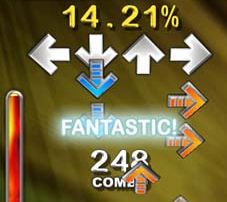
\includegraphics[width=0.25\textwidth]{protagonist.png}
	\end{center}
	\caption{ITG gameplay, including score indicator (top), protagonist avatar (mid), directional obstacles (low), and step judgement, life bar, and combo indicator (figure these out for yourself).}
	\label{fig:protagonist}
\end{figure}
\begin{figure}[t]
	\begin{center}
	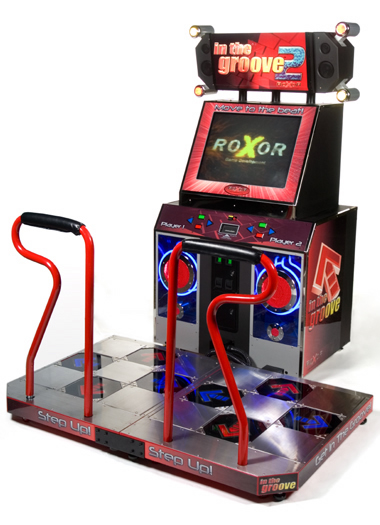
\includegraphics[width=0.2\textwidth]{itg2cabinet.jpg}
	\end{center}
	\caption{An ITG cabinet. RIP in Peace, Roxor.}
	\label{fig:cab}
\end{figure}

The game may be played in several modes, the most common of which supports up to two (2) players, each operating their own protagonist using either the left or right set of four arrows.
This game mode may be played with or without the assist of a curved metal rod mounted behind the arrows (henceforth, ``bar''), as shown in Figure~\ref{fig:bengreg}.
In other game modes, a single player may operate up to all 8 of the arrows. When all 8 are used, the game mode is known as ``Doubles'', as shown in Figure~\ref{fig:jim}, and is often associated with excessive No-Barring, use of hands and knees to operate the arrows, and impressive facial hair.
In this body of work, we will focus exclusively on the Singles game mode, in which each player controls four arrows: one Up ($U$), one Down ($D$), one Left ($L$), and one Right ($R$). Without loss of generality, we further assume that only one player plays at a time, and that she or he will shower immediately afterward.

\begin{figure}[t]
	\begin{center}
	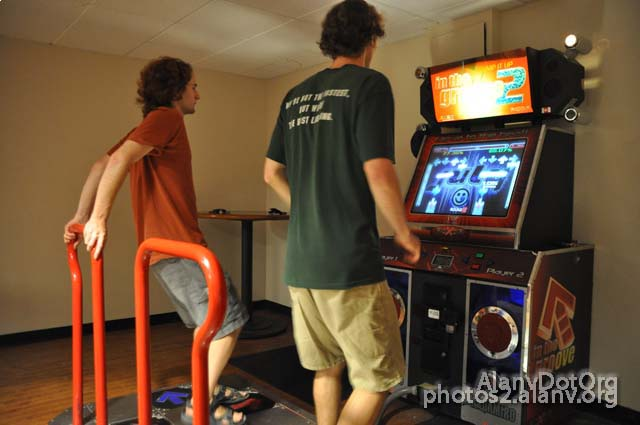
\includegraphics[width=0.48\textwidth]{bengreg.jpg}
	\end{center}
	\caption{ITG can be played ``Bar'' or ``No-Bar''. Bar players must wear sandals (like an idiot; who is that guy anyway?), while No-Barrers must always play on the right.}
	\label{fig:bengreg}
\end{figure}
\begin{figure}[t]
	\begin{center}
	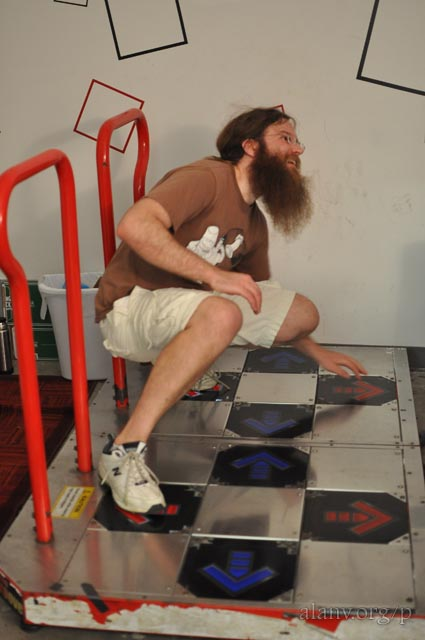
\includegraphics[width=0.25\textwidth]{jim.jpg}
	\end{center}
	\caption{Doubles play is beyond the scope of our work. It requires (or perhaps produces?) a magnificent beard.}
	\label{fig:jim}
\end{figure}

\bibliographystyle{alpha}
\bibliography{paper}

%\onecolumn
%
%\appendix


\end{document}
